%%% File encoding: UTF-8

%%% Magic comments for setting the correct parameters in compatible IDEs
% !TeX encoding = utf8
% !TeX program = pdflatex 
% !TeX spellcheck = en_US
% !BIB program = biber

\RequirePackage[utf8]{inputenc} % Remove when using lualatex or xelatex!
\RequirePackage{hgbpdfa}        % Creates a PDF/A-2b compliant document

\documentclass[type=bachelor,theme=default,language=english,titlelanguage=english,smartquotes]{hgbthesis}
% Supported options in [..]: 
%    Type of work (type=): 'master' (default), 'bachelor', 'diploma', 'phd', 'internship'
%    Title page theme (theme=): 'default' (default), 'fhooe24'
%    Use as thesis proposal: 'proposal' or 'proposal=true' 
%    Main document language (language=): 'german' (default), 'english'
%    Title page language (titlelanguage=): 'german', 'english' (default is main language)
%    Conversion to typographic quotation marks: 'smartquotes'
%    Use APA citation style: 'apa'
%    Page layout: 'oneside' (single-sided, default), 'twoside' (double-sided)
%%%-----------------------------------------------------------------------------

\graphicspath{{images/}}  % Location of images and graphics
\bibliography{references} % Biblatex bibliography file (references.bib)

%%%-----------------------------------------------------------------------------
\begin{document}
%%%-----------------------------------------------------------------------------

%%%-----------------------------------------------------------------------------
% Title page entries
%%%-----------------------------------------------------------------------------

\title{InpaintAR}
\subtitle{A Comparison of different InPainting Approaches for Real-Time Use}
\author{Sebastian Gradwohl}

\programtype{Bachelor's Degree Program} % or Bachelor's Degree Program
\programname{Software Engineering}
\institution{University of Applied Sciences Upper Austria}

\placeofstudy{Hagenberg}
\dateofsubmission{2026}{02}{01} % {YYYY}{MM}{DD}

% List of advisors, up to 4 are possible, title in [] is optional
\advisor{FH-Prof. Dr. Christoph Anthes, MSc}
%\advisor[Second Advisor]{FH-Prof.\textsuperscript{in} Susanna A.~D. Visor, PhD}

\license{cc}      % Publish under Creative Commons License (recommended)
%\license{strict} % Restrictive license, "all rights reserved"

%%%-----------------------------------------------------------------------------
\frontmatter                                   % Front part (roman page numbers)
%%%-----------------------------------------------------------------------------

\maketitle
\tableofcontents

\chapter{Preface} % German: Vorwort

This is version \textbf{\hgbDate} of the \latex document template for various
theses at the School of Informatics, Communication and Media at the University
of Applied Sciences Upper Austria in Hagenberg. We are pleased to learn that this
document collection is meanwhile also used at various other institutions in Austria
and abroad.

The document was initially created in response to requests from students after
the 2000/01 academic year when an official \latex introductory course was
offered in Hagenberg for the first time. The fundamental idea was to
"simply" convert the already existing \emph{Microsoft Word} template for
diploma theses to \latex\ and possibly to add some unique features. This quickly
turned out to be not very useful since \latex, especially concerning the
handling of literature and graphics, requires a substantially different way of
working. The result is--- rewritten from scratch and much more extensive than
the previous document---a manual for writing with \latex, supplemented with
additional (meanwhile removed) hints for \emph{Word} users. Technical details
of the current version can be found in Appendix \ref{app:TechnicalDetails}.

While this document was initially intended exclusively for the preparation
of diploma theses, it now also covers \emph{master theses},
\emph{bachelor theses}, and \emph{internship reports}. The differences between
these documents have been deliberately kept small.


When creating this template, an attempt was made to work with the basic
functionality of \latex and---as far as possible---to achieve this without
additional packages. This was only partially successful; several supplementary
"packages" are necessary, but only common extensions have been used. Of course,
there is a large number of additional packages which can be helpful for further
improvements and refinements. Everyone is encouraged to experiment with these as
soon as they have the necessary self-confidence and sufficient time to
experiment. Many details and tricks are not explicitly mentioned in this
document but can be explored in the underlying source code at any time.

Numerous colleagues have provided valuable support through careful proofreading
and constructive suggestions for improvement. We thank Heinz Dobler for
consistently improving our "computer slang" and Elisabeth Mitterbauer for her
proven "orthographic eye".

Usage of this template is free without any restrictions and not bound to any
mention. However, when used as a basis for one's work, one should not simply
start working on it, but at least \emph{read} the essential parts of the
document and, if possible, take them to heart. Experience has shown that this
improves the quality of the results significantly.

This document and the associated \latex classes have been available since
November 2017 on CTAN%
\footnote{Comprehensive TeX Archive Network} 
as package \texttt{hagenberg-thesis},
%
\begin{itemize}
	\item[]\url{https://ctan.org/pkg/hagenberg-thesis}.
\end{itemize}
%
The current source code, as well as additional materials---such as a wiki with
instructions for the integration of often requested functionalities and
extensions---can be found at
%
\begin{itemize}
  \item[]\url{https://github.com/Digital-Media/HagenbergThesis}.%
  \footnote{\url{https://github.com/Digital-Media/HagenbergThesis/blob/main/CHANGELOG.md}
  contains a list of chronological changes (formerly included in the appendix
  of this document).}
\end{itemize}

\noindent
Despite great efforts, a document like this always contains errors and
shortcomings. Comments, suggestions, and helpful additions are welcome.
Ideally, as comments or issues on GitHub.

By the way, here, in the preface (which is common in diploma and master theses
but dispensable for bachelor's theses), you may briefly describe the genesis of
the document. This is also the place for any acknowledgments (\eg, to the
supervisor, the examiner, the family, the dog, \etc) as well as dedications and
philosophical remarks. These should be balanced and limited to a maximum of two
pages.

\vspace{6ex}
\noindent
W.\ Burger (em.) and W.\ Hochleitner\\[1ex]
University of Applied Sciences Upper Austria\\ 
Department of Digital Media, Hagenberg\\
\url{https://www.fh-ooe.at/campus-hagenberg/}
 % A preface is optional
\chapter{Abstract}

Large Public Display Games place several specific design requirements. Such
games need to work equally well for just a few or several simultaneous users.
Also, entering, leaving, or joining a game in progress should be easily possible
without interrupting the game's flow. This bachelor (master) thesis focuses on
developing a game mechanics framework that supports the principle of smooth
transition gameplay. This framework will then be evaluated utilizing a prototype
implemented in a term project.
		
\chapter{Kurzfassung}

\begin{german}
Aufgrund der technologischen Fortschritte, sowohl in der Hardware, als auch in der Software-Integration, steigt die Beliebtheit von Augmented Reality mit jedem Jahr an.
\\
Ein sehr gängiges Problem in aktueller Augmented Reality Software ist die Ablenkung, welche durch physische Objekte, die um den digitalen Inhalten liegen. Beispielsweise bei der immersiven Analyse von Daten.
\\\\
In dieser Bachelorarbeit liegt der Fokus auf der Analyse verschiedener Methoden und Algorithmen zur Verdeckung dieser Objekte, wodurch eine aufgeräumte, saubere Umgebung für die digitalen Elemente geschaffen wird.
\\
Um dies zu erreichen wird ein Werkzeug entwickelt, welches erlaubt Flächen zu wählen, welche dann dazu verwendet werden, um Objekte auf diesen Flächen zu finden und darauffolgend durch die Nutzung von Inpainting zu verdecken. Mithilfe dieses Werkzeugs werden mehrere Methoden und Algorithmen sowohl auf Qualität, als auch auf Leistung evaluiert, um sowohl die Glaubbarkeit und Ordnung der generierten Umgebungen, während parallel dazu ein Fokus auf die Minimierung von Rechenresourcen und Laufzeit gelegt wird.
\\
Diese Ergebnisse werden zueinander verglichen, sodass Leser sowohl über die Vor- als auch Nachteile der jeweiligen Ansätze einen Überblick bekommen.
\end{german}			

%%%-----------------------------------------------------------------------------
\mainmatter                                    % Main part (arabic page numbers)
%%%-----------------------------------------------------------------------------

\chapter{Introduction}
\label{cha:Introduction}

The Domain of Augmented Reality (AR)  spans all kinds of real-time visualization approaches wherein an otherwise real environment gets augmented with virtual objects \cite{Milgram1994}
While many still consider Augmented Reality a nieche, the user-numbers tell a different story. In 2023 Statista reported about 983 Million users to be using AR on their mobile devices. This number is set to grow to 1.187 Billion users until 2028 \cite{Statista2024}.

One of the issues still common in AR Applications is the overload of information. Whenever users are supposed to focus on the virtual objects at hand, the visibility of physical objects may serve as a distraction. (cf. Cheng et. al. \cite{ChengYiFei2022TUDR})
An existing solution is the use of Diminished Reality. This Concept aims to hide certain physical objects from the viewport, which can in this case be used to reduce the visual clutter.

\section{Motivation}

While there are many existing solutions for achieving Diminished Reality using Inpainting , the topic of which inpainting method for not only this usecase, but Inpainting in a 3-Dimensional Real-Time Environment has largely been disregarded as of now. Most Papers put the focus on different components of the system like the detection of the objects, user studies or optimizations of smaller visual artifacts.
Over the last years there have been numerous achievements in the space of Inpainting methods, ranging from low-cost, small area optimized algorithms like the fast marching algorithm \cite{Weiwei2021} to machine-learning assisted large area approaches like the DeepFill Deep-Learning model.\cite{MuziHao2023}

The main goal of this analysis is to provide an easy to reference comparison of the different methodologies to be compared in terms of both performance and quality. Through this analysis, developers can make an educated choice on which methodology to use for their usecase, be it high fidelity in usecases like PC-Powered AR Systems or low energy, low performance systems, more suited for mobile devices, be they mobile phones or standalone Mixed-Reality Head-Mounted Displays.
In addition, the tool built for this evaluation should be easy to extend for newer inpainting methods whilst staying easy to integrate into existing applications.

\section{Overview}

This work includes an introduction to the underlying concepts and analyzed inpainting methods, followed by the conceptualization and implementation of the tool as well as the performance and quality evaluation for each of the analyzed inpainting methods. These topics are elaborated upon in the following five chapters:

\begin{itemize}
\item Chapter 2: Fundamentals and Related Work
Provides an introduction into visual clutter and why it matters to the domain of Augmented Reality, an introduction to the term of Diminished reality aswell as the underlying logic of each of the inpainting methods. 

\item Chapter 3: Concept
Elaborates on the architecture and design chosen for this tool and provides an overview on a few example usecases for which the tool might be used

\item Chapter 4: Implementation
The focus lies on providing an explanation on each of the classes contained in this tool and how it can be implemented into existing projects to be used. In Addition some of the tools and principles used during the implementation are going to be elaborated on.

\item Chapter 5: Evaluation
After providing an overview of the testing setup and how visual clutter and performance are measured, the test scenarios will be presented, followed by the results for each of the analyzed methods.

\item Chapter 6: Conclusion
Presents the findings of the evaluation in a summed up manner and goes into detail on how the tool might be expanded in the future to improve the tool to provide an even better user and developer experience
\end{itemize}
%\chapter{Writing a Thesis}
\label{cha:TheThesis}

Every thesis%
\footnote{Most of the following remarks apply equally to bachelor's, master's,
and diploma theses.}
is different, yet good theses are usually very similar in structure, especially
in the fields of engineering and natural sciences.

\section{Elements of a Thesis}

The following basic structure has proven itself as a starting point, which can,
of course, be varied and refined as desired:
%
\begin{enumerate}
	\item \textbf{Introduction and motivation}: What is the problem statement or
	task at hand, and why should someone be interested in it?
	\item \textbf{Speficiation of the topic in greater detail}: Here, the
	current state of the art of the technology or science is described, and
	existing deficits or open questions are pointed out. The direction of one's
	work is developed from this.
	\item \textbf{Own approach}: This is, of course, the core of the thesis.
	Here it is shown how the previously described task is solved and
	implemented, often in the form of a prototype. Illustrative examples
	supplement this part.
	\item \textbf{Summary}: What has been achieved, and what goals remain open?
	Which parts of the thesis are possible origins for further work?
\end{enumerate}
%
Of course, a certain dramaturgical structure of the thesis is also important.
Remember that readers usually have little time and---unlike in a novel---their
patience should not be tried. Explain already in the introduction (not in the
last chapter) how you approached the problem, your proposed solutions, and if
you successfully applied them.

Errors and dead ends may (and should) be described as well; their knowledge
often helps to avoid duplicate experiments and other errors and is thus
certainly more helpful than any whitewashing. And, of course, it is acceptable
to express one's own ideas and opinions as long as they are rationally stated.


\section{Language and Writing Style}

A thesis is a piece of scientific work and should therefore be formulated concisely 
and factually. The author's person takes a back seat to the subject of the
work; avoid the first person or wordings such as "the author". Passive voice can
be a remedy, although it is vital to ensure that this does not result in an
overly complicated sentence structure. Also, remember that the active voice
makes writing sound stronger and more direct and helps to deliver essential
aspects more precisely.

Expressions such as colloquialisms, polemical formulations, or even irony and
cynicism are out of place, as is the excessive use of overly specific technical
terms.

Furthermore, the language used in a thesis should be gender-inclusive and
non-discri\-minatory, making all people equally visible in their diversity,
both in words and images. In English, this includes using nouns that are not
gender-specific to refer to roles or professions, formation of phrases in a
coequal manner, and avoiding the blanket use of male or female terms.

Avoid gender-specific job titles such as "fireman" or "stewardess" and replace
them with the more neutral terms "firefighter" or "flight attendant". When
using pronouns, refrain from using "he" or "she". Replace these with the more
inclusive "they" to include people who identify as non-binary.

Also, check the writing for terms that might be considered racially
inappropriate. Expressions such as "master" and "slave" or "whitelist" and
"blacklist" might be considered offensive by certain groups of people. Keep this
in mind when naming things in the project or prototype. Especially in a
scientific thesis, the potential of language should be used to counter
stereotypical ideas about social roles.


\section{Writing a Thesis in English at a German-Speaking University}
\label{sec:german}

While this template and the contained introduction should make it easy to write
a thesis entirely in English, there are still some things that have to remain in
German, should the University demand it.

The title page must usually be German and stays the same when the document is
set to English. Also, a German Kurzfassung is required together with the English
Abstract. Using a translator is a valid option for everyone who is not fluent
in German. Having the translation checked by a native German speaker is
recommended, however.

The German term "Fachhochschule" (as in Fachhochschule Oberösterreich) is
translated with "University of Applied Sciences". A master's thesis is called
"Masterarbeit," and a bachelor's thesis is called "Bachelorarbeit".

If one's native language is German, it should be considered that writing a
thesis in English (unless the program requires it) does not make writing any
easier, even if it might feel that way at first. Particularly in computer
science, the dominance of English technical terms makes writing in German seem
tedious, and switching to English might appear particularly attractive. However,
this is deceptive since one's skill in a foreign language is often overestimated
(despite the usually long years of English education). Conciseness and clarity
are easily lost, and sometimes the result is an embarrassing drivel without
context and solid content. Unless one's English skills are excellent, writing at
least the most essential parts of the thesis in German first and only
translating them afterward is advisable. Special care should be taken when
translating seemingly familiar technical terms. In addition, it is always
helpful to have the finished work checked by a native speaker.

Parallel to this document, there is also a German version, which is largely
identical in content. It contains helpful hints for writing a thesis in German
and should be used if German is the language of choice. Technically, except for
the language setting and the different quotation marks (see
Section~\ref{sec:quotation-marks}), there is nothing more to consider to use
this template in German.


\section{Making Use of AI Tools}

Artificial intelligence (AI) tools are now widely used for writing texts, this
includes academic writing. Many of these applications are based on so-called
\emph{large language models} (LLMs) that have been trained on huge amounts of text.
Through statistical analyses of millions or billions of words, these models
learn to highly likely to generate meaningful sentences and recognize
connections. Examples of AI-supported writing assistants include 
ChatGPT\footnote{\url{https://chatgpt.com/}},
DeepL Write\footnote{\url{https://www.deepl.com/write}} or 
Grammarly\footnote{\url{https://grammarly.com/}}.

When writing a thesis, AI tools can help make existing texts more efficient,
for example, by checking spelling and grammar, improving style and readability,
or suggesting initial wording. This saves time and allows the author to focus
more on the content quality and the work's structure.

At the same time, such tools also entail risks. In particular, they
\textbf{should not} be used to generate new content. There is a risk that
incorrect texts may be created or findings uncritically adopted. Furthermore,
AI models can reproduce prejudices or use lines of argument that contradict a
thorough scientific approach. Last but not least, a text generated by an AI
tool is not (as can be seen, for example, in the declaration of the documents
generated with this template) "the result of [one's] own original work", which
goes against the idea of a thesis as an independent academic achievement.

\subsection{Important Points When Using AI Tools}

\begin{itemize}
	\item Use AI tools in the text only to revise the wording or to make
	linguistic improvements.
	\item Document the use of AI assistants if large parts of the text or
	revisions have been created with the help of such a tool.
	\item This documentation can be done, for example, by adding a note in a
	footnote or at the beginning of a section. It is helpful to specify the
	prompt used if it goes beyond a simple "revise this paragraph".
	\item Adding a reference with the AI tool as the author should be avoided
	since the results are not deterministic.
	\item For AI-generated media (\eg, images) specifiy the tool used, and the
	prompt in the caption. See Section \ref{sec:SourceCitationsInCaptions}.
	\item The responsibility for the AI content used always lies with the
	author. It is therefore important to critically review, question, and, if
	necessary, correct the results.
\end{itemize}

%\chapter{Working with \latex}
\label{cha:WorkingWithLatex}


%\chapter{Figures, Tables, Source Code}
\label{cha:Figures}

%\chapter[Mathematical Formulas etc.]{Mathematical Formulas, Equations and Algorithms}
\label{cha:Mathematics}


Typesetting mathematical elements is certainly one of the strongest features of
\latex. A distinction is made between mathematical elements in continuous text
and free-standing equations, which are usually numbered consecutively.
Analogous to figures and tables, this makes it easy to cross-reference equations.
Here are only some examples and special topics, much more can be found in 
\cite[Ch.\ 7]{Kopka2003} and~\cite{Voss2014}.


\section{Mathematical Elements in Continuous Text}

Mathematical symbols, expressions, equations, etc.\ are marked in the continuous
text by pairs \verb!$! \ldots \verb!$!. Here is an example:
%
\begin{quote}
	%\item[]
	The near infinity point is at $\bar{a} = f \cdot (f / (K \cdot u_{\max}) + 1)$, 
	so with a lens set to $\infty$, everything is in focus from distance $\bar{a}$ on.
	Focusing the lens to the distance $\bar{a}$ (\ie, $a_0 = \bar{a}$), everything
	in the range $[\frac{\bar{a}}{2}, \infty]$ will be in focus.
\end{quote}
%
It is important to ensure that the height of the individual math items in the text
does not become too large.

\subsubsection{Common Mistakes}

In continuous text, simple variables are often typeset with plain text,
\ie, without using correct mathematical symbols, as in "X-axis" instead of 
"$X$-axis" (\verb!$X$-axis!).


\subsubsection{Mathematical Fonts}

\latex\ uses slightly different fonts for regular text and in math mode.
The following basic math fonts are available:
%
\begin{quote}
    \begin{tabular}{lcl}
        $\mathrm{Roman}$      & & \verb!$\mathrm{Roman}$!,      \\
				$\mathit{Italic}$     & & \verb!$\mathit{Italic}$!,      \\
				$\mathbf{Bold}$     	& & \verb!$\mathit{Bold}$!,      \\
        $\mathsf{Sans Serif}$ & & \verb!$\mathsf{Sans Serif}$!, \\
        $\mathtt{Typewriter}$ & & \verb!$\mathttt{Typewriter}$!, \\
				$\mathcal{CALLIGRAPHIC}$ & & \verb!$\mathcal{CALLIGRAPHIC}$!,\\
				$\mathbb{BLACKBOARD}$ & & \verb!$\mathbb{BLACKBOARD}$!,\\
				$\mathfrak{Fraktur}$ & & \verb!$\mathfrak{Fraktur}$!.
    \end{tabular}
\end{quote}
%
In some situations, the \verb!\boldsymbol{..}! macro may come in useful. It can 
convert any mathematical symbol into a boldface version, for example,
$\mathbf{A}$ (\verb!$\mathbf{A}$!) denotes a matrix and $\boldsymbol{x}$ 
(\verb!$\boldsymbol{x}$!) is a vector.


\subsubsection{Line Breaks}

With longer mathematical elements in the continuous text problems with line breaks 
are inevitable. Usually \latex allows line breaks only at the "=" operator, 
elsewhere one can use \verb|\allowbreak| to enable line breaks. Here is a small
example:
%
\begin{itemize}
	\item[a)] For example, (bla bla bla) a simple row vector is defined in the form
	$\boldsymbol{x} = (x_0, x_1, \ldots, x_{n-1})$.
	\item[b)] For example, (bla bla bla) a simple row vector is defined in the form
	$\boldsymbol{x} = (x_0,\allowbreak x_1,\allowbreak\ldots,\allowbreak
	x_{n-1})$.
\end{itemize}
%
The line in a) should extend beyond the page margin, but b) contains 
\verb|\allowbreak| in several places and should therefore wrap cleanly.


\section{Displayed Expressions and Equations}

Displayed mathematical expressions can be generated in \latex\ by \verb!\[! \ldots 
\verb!\]! The result will be centered, but will not be numbered.
For example, \[y_0 = 4 x^2\] is produced by \verb!\[y_0 = 4 x^2\]!
or, alternatively,
%
\begin{LaTeXCode}[numbers=none]
\begin{displaymath} y_0 = 4 x^2 \end{displaymath}
\end{LaTeXCode}



\subsection{Numbered Equations}

However, most often in such cases the \texttt{equation} environment is used
to produce numbered equations that can be referred to at any time in the text.
For example, 
%
\begin{LaTeXCode}[numbers=none]
\begin{equation}
	f(k) = \frac{1}{N} \sum_{i=0}^{k-1} i^2 .
	\label{eq:MyFirstEquation}
\end{equation}
\end{LaTeXCode}
%
creates this equation:
%
\begin{equation}
	f(k) = \frac{1}{N} \sum_{i=0}^{k-1} i^2 .
	\label{eq:MyFirstEquation}
\end{equation}
%
With \verb|\ref{eq:MyFirstEquation}| you get the number (\ref{eq:MyFirstEquation})
of this equation as usual (see also Section~\ref{sec:ReferencesToEquations}).
The same equation \emph{without} numbering can be generated with the \texttt{equation*}
environment.
%
\begin{center}
	\setlength{\fboxrule}{0.2mm}
	\setlength{\fboxsep}{2mm}
	\fbox{%
		\begin{minipage}{0.9\textwidth}
		Note that \emph{equations} are a \emph{part of the main text} in terms of content, 
		and therefore, in addition to proper linguistic \emph{transitions},
		\emph{punctuation} (as shown in Equation \ref{eq:MyFirstEquation}) must be observed.
		If you are unsure, you should look at suitable examples in a good math textbook.
		\end{minipage}}
\end{center}
%
For those interested, more on the intimate connection between mathematics and prose can
be found in \cite{Mermin1989} and \cite{Higham2020}.


\subsection{Multiline Equations}

For multiline equations \latex\ offers the \verb!eqnarray! environment which, however,
generates somewhat idiosyncratic spacing. It is recommended to use the extended
possibilities of the \texttt{amsmath} package%
\footnote{American Mathematical Society (AMS). \texttt{amsmath} is part of the 
\latex\ default installation and is automatically imported by \texttt{hgb.sty}.}
for this right away. Here is an example with two equations aligned to the $=$ sign,
%
\begin{align}
	f_1 (x,y) &= \frac{1}{1-x} + y , \label{eq:f1} \\
	f_2 (x,y) &= \frac{1}{1+y} - x , \label{eq:f2}
\end{align}
%
generated with the \texttt{align} environment from the \texttt{amsmath} package:
%
\begin{LaTeXCode}[numbers=none]
\begin{align}
  f_1 (x,y) &= \frac{1}{1-x} + y , \label{eq:f1} \\
  f_2 (x,y) &= \frac{1}{1+y} - x , \label{eq:f2}
\end{align}
\end{LaTeXCode}


\subsection{Multi-Case Constructs}

With the \texttt{cases} environment from \texttt{amsmath}, case distinctions, 
\eg, in function definitions, are very easy to accomplish.
For instance, the recursive definition
%
\begin{equation}
	f(i) =
	\begin{cases}
		0             & \text{for $i = 0$,}\\
		f(i-1) + f(i) & \text{for $i > 0$.}
	\end{cases}
\end{equation}%
%
was produced with the following commands:
%
\begin{LaTeXCode}[numbers=none]
\begin{equation}
	f(i) =
	\begin{cases}
	  0             & \text{for $i = 0$,}\\
	  f(i-1) + f(i) & \text{for $i > 0$.}
	\end{cases}
\end{equation}
\end{LaTeXCode}
%
Note the use of the very handy \verb!\text{..}! macro, which can be used
to insert ordinary text in math mode, and again the punctuation within the
equation.


\subsection{Equations With Matrices}

Again, \texttt{amsmath} offers some advantages over using the standard \latex
constructs. For this purpose, a simple example of using the \texttt{pmatrix}
environment for vectors and matrices,
%
\begin{equation}
	\begin{pmatrix}
		x' \\ y'
	\end{pmatrix}
	=
	\begin{pmatrix}
		\cos \phi & -\sin \phi           \\
		\sin \phi & \phantom{-}\cos \phi
	\end{pmatrix}
	\cdot
	\begin{pmatrix}
		x \\ y
	\end{pmatrix} ,
\end{equation}
%
generated with the following instructions:
%
\begin{LaTeXCode}
\begin{equation}
	\begin{pmatrix} 
			x' \\ 
			y' 
	\end{pmatrix}
	= 
	\begin{pmatrix}
		  \cos \phi &          -\sin \phi \\
		  \sin \phi & \phantom{-}\cos \phi /+ \label{lin:phantom} +/
	\end{pmatrix} 
	\cdot
	\begin{pmatrix} 
			x \\ 
			y 
	\end{pmatrix} ,
\end{equation}
\end{LaTeXCode}
%
A useful detail in this is the \tex macro \verb!\phantom{..}! (in line 
\ref{lin:phantom}), which inserts its argument invisibly and is used here
as a placeholder for the minus sign above it.
As an alternative to \texttt{pmatrix}, the \texttt{bmatrix} environment can
be used to create matrices and vectors with square brackets.
Numerous other mathematical constructs of the \texttt{amsmath} package are
described in \cite{Mittelbach2024}.


\subsection{References to Equations}
\label{sec:ReferencesToEquations}

When referring to numbered formulas and equations, it is usually sufficient
to indicate the corresponding number in round brackets, \eg,
%
\begin{center}
	"\ldots\ as can be derived from (\ref{eq:f1}) \ldots"
\end{center}
%
To avoid misunderstandings, however---especially in texts with only few
mathematical elements---"Equation \ref{eq:f1}", "Eq.~\ref{eq:f1}" or 
"Eq.~(\ref{eq:f1})" should be written (consistently, of course).
%
\begin{center}
	\setlength{\fboxrule}{0.2mm}
	\setlength{\fboxsep}{2mm}
	\fbox{%
		\begin{minipage}{0.9\textwidth}
			Note: Forward references to equations (placed further back
			in the text) are \emph{extremely uncommon} and should be avoided! If
			one still believes to need such a thing, then usually a mistake was made
			in the content structure.
		\end{minipage}}
\end{center}


\section{Mathematical Symbols}

Special macros are needed for a large part of the mathematical symbols. Some of
the most common ones are listed  in the following.


\subsection{Number Sets}

Some frequently used symbols are unfortunately not included in the original 
mathematical character set of \latex, suchh as the symbols for the real and natural 
numbers. In the \texttt{hagenberg-thesis} package these symbols are defined
as macros%
\footnote{Based on the \emph{AMS Blackboard Fonts}.}
\verb!\R!, \verb!\Z!, \verb!\N!, \verb!\Cpx!, \verb!\Q! ($\R, \Z, \N, \Cpx, \Q$),
\eg,
%
\begin{center}
	$x \in \R$ , $k \in \N_0$, $z = (a + \mathrm{i} \cdot b) \in \Cpx$.
\end{center}


\subsection{Operators}

In \latex\ dozens of mathematical operators are defined for various purposes.
Of course, the arithmetic operators $+$, $-$, $\cdot$ and $/$ are needed most often.
A frequent mistake (probably resulting from programming practice) is the use
of $*$ for simple multiplication---correct is $\cdot$ (\verb!\cdot!).%
\footnote{The $*$ character is usually reserved for the \emph{convolution operator}.}
%
For statements like "a field with $25 \times 70$ meters" (but also almost
\emph{only} for that) it makes sense to use the $\times$ (\verb!\times!) operator
-- and \emph{not} simply the text character~"x"!


\subsection{Variables (Symbols) With Multiple Characters}

Especially in the mathematical specification of algorithms and programs
it is often necessary to use symbols (variable names) with more than one
character, \eg,
%
	\[Scalefactor\leftarrow p^2 \cdot 1.5 \; ,\]
%
\emph{falsely} implemented by
%
\begin{LaTeXCode}[numbers=none]
$Scalefactor \leftarrow Scalefactor^2! \verb!\cdot 1.5$
\end{LaTeXCode}
%
The reason is that \latex interprets the character sequence "Scalefactor" as
the product of 11 single, consecutive variables $S$, $c$, $a$, $l$, $e$, \ldots
and inserts appropriate spaces between them.
The \emph{correct} way is to combine these letters with \verb!\mathit{..}! to 
\emph{one} symbol. The difference is clearly visible in this case:
%
\begin{center}
	\setlength{\tabcolsep}{4pt}
	\begin{tabular}{llll}
		\text{Wrong:}  & $Scalefactor^2$          & $\leftarrow$ &
		\verb!$Scalefactor^2$!          \\
		\text{Correct:} & $\mathit{Scalefactor}^2$ & $\leftarrow$ &
		\verb!$\mathit{Scalefactor}^2$!
	\end{tabular}
\end{center}
%
Generally, such long symbol names should be avoided anyway and short symbols
used instead wherever possible (\eg, focal length $f = 50 \, \mathrm{mm}$ 
instead of $\mathit{focal length} = 50 \, \mathrm{mm}$).


\subsection{Functions and Operators}

While symbols for variables are traditionally (and in \latex\ automatically)
set \emph{italic}, names of functions and operators are usually typeset in
\emph{roman} fonts, as for example in
%
\begin{center}
	\begin{tabular}{lcl}
		$\sin \theta = \sin(\theta + 2 \pi)$ &
		$\leftarrow$ & \verb!$\sin \theta = \sin(\theta + 2 \pi)$! \\
	\end{tabular}
\end{center}
%
This happens with the already predefined standard functions (like \verb!\sin!, 
\verb!\cos!, \verb!\tan!, \verb!\log!, \verb!\max! \uva) automatically.
This convention should also be followed for self-defined functions, such as in
%
\begin{center}
	\begin{tabular}{lcl}
	$\mathrm{dist}(A,B) := |A-B|$ & $\leftarrow$ & 
	\verb!$\mathrm{dist}(A,B) := |A-B|$! \\
	\end{tabular}
\end{center}


\subsection{Units of Measurement and Currencies}

When specifying units of measurement, normal font is usually used (no italics) 
should be used, \eg:
%
\begin{quote}
	The maximum speed of the \textit{Bell XS-1} is 345\,m/s with a takeoff weight 
	of 15\,t. The prototype cost over US\$ 25,000,000, or about \euro 19,200,000
	in today's conversion.
\end{quote}
%
The blank space between the number and the unit of measurement is intentional.
The \$ sign is created with \verb!\$! and the Euro symbol (\euro) is created
with the \verb!\euro! macro.%
\footnote{The \euro symbol is not included in the original \latex character 
set but is provided by the \texttt{marvosym} package (\texttt{{\bs}EUR}).}


\subsection{Commas in Decimal Numbers (Math Mode)}


In math mode (\ie, within \verb!$! \ldots \verb!$!, \verb!\[! \ldots \verb!\]! or 
in equations) \latex\ generally follows the Anglo-American convention that 
\emph{dot} (\verb!.!) is used as the comma sign decimal numbers.
For example, \verb!$3.141$! produces the output "3.141", as one would expect.
Unfortunately, to use a European comma in decimal numbers, it is \emph{not}
sufficient to simply replace \verb!.! with \verb!,!.
In this case the comma is interpreted as \emph{punctuation character} and 
the result looks like this:
%
\begin{quote}
	\verb!$3,141$! $\quad \rightarrow \quad 3,141$
\end{quote}
%
(note the additional blank space after the comma). This behavior can be
redefined globally in \latex, but this in turn leads to a number of unpleasant
side effects. A simple (though not very elegant) solution is to write decimal
numbers in math mode like this:
%
\begin{quote}
	\verb!$3{,}141$! $\quad \rightarrow \quad 3{,}141$
\end{quote}


\subsection{Mathematical Tools}

For the creation of complicated equations it is sometimes helpful to resort 
to special software or interactive tools. Among other things, \latex statements
for mathematical equations can be exported from Microsoft's \emph{Equation Editor}
or \emph{Mathematica} in a relatively simple way and copied directly (usually
with some manual rework) into your own \latex document.


\section{Algorithms}


Algorithmic representations are an important means of accurately describing
computational processes. By using \emph{mathematical notation} (symbols and 
operators) on the one hand and the \emph{sequence structures} (decisions, 
loops, procedures, \etc) familiar from programming, algorithms are a proven 
link between the mathematical formulation and the associated program code.

An essential aspect of an algorithmic description---which should be
structurally as similar as possible to the implementation--- is its
\emph{independence} from a specific programming language.
This results in better readability, broader applicability, and increased
sustainability (possibly beyond the lifetime of a programming language).
When formulating algorithms, one should consider the following, among other
things:%
\footnote{See also
\url{http://mirrors.ctan.org/macros/latex/contrib/algorithms/algorithms.pdf}
(Section~7).}
%
\begin{itemize}
	\item
	Use the same short symbols (such as $a, i, x, S, \alpha \ldots$) in
	algorithms as you would in mathematical definitions and equations.
	\item
	If possible, use proper \emph{mathematical} operators, such as 
  $=$, $\leq$, $\cdot$, $\wedge$ \etc,
  instead of the associated programming constructs 
  \texttt{==}, \texttt{<=}, \texttt{*}, \texttt{\&\&}, respectively.
  %
	%$=$ (\verb!$=$!) for \texttt{==}, \texttt{*}
	%$\leq$ (\verb!$\leq$!) for \texttt{<=},
	%$\cdot$ (\verb!$\cdot$!) for \texttt{*}, 
	%$\wedge$ (\verb!$\wedge$!) for \texttt{\&\&},
	%\etc
	\item
	Similarly. do not use elements or syntax of a specific programming language (for
	example, a "\texttt{;}" at the end of a statement is unnecessary).
	\item
	If an algorithm becomes too long for a page, consider how to divide it
	sensibly into smaller modules (perhaps the associated program structure
	is not optimal either).
\end{itemize}

\noindent
For the notation of algorithms in mathematical form or even for pseudocode,
no special support is provided in \latex itself. However, there are several
useful \latex packages for this purpose, including \texttt{algorithmicx},
 which is also used here because of its simple syntax, but in the improved
version \texttt{algpseudocodex}.%
\footnote{Style \nolinkurl{hgbalgo.sty} of \texttt{hagenberg-thesis}
extends the packages \texttt{algorithmicx} and \texttt{algpseudocodex} 
(see \url{https://ctan.org/pkg/algpseudocodex}) by providing improved
indentation, colors, \etc}
%
The example in Algorithm~\ref{alg:Example} was created using the float
environment \texttt{algorithm} and the \texttt{algpseudocodex} package (see the
source code in Program~\ref{prog:AlgExample}). For better readability, vertical
rules are used (\texttt{indLines=true}) and the optional keyword 
"\texttt{end}" at the end of blocks is omitted (\texttt{noEnd=true}).


%%--------------------------------------------------------------------

\begin{algorithm}
\caption{Example of an algorithm for bicubic interpolation in 2D 
\cite{BurgerBurge2022}, typeset with package \texttt{algpseudocodex}.
Function $\Call{Cubic1D}{x}$, used in lines \ref{alg:wcub1} and 
\ref{alg:wcub2}, calculates the weight given to the interpolation value at 
some one-dimensional position $x$.}
\label{alg:Example}

\begin{algorithmic}[1]     % [1] = all lines are numbered
\Function{BicubicInterpolation}{$I, x, y$} \Comment{two-dimensional interpolation}
	\Input{$I$, original image; $x,y \in \R$, continuous position.}
	\Returns{the interpolated pixel value at position $(x,y)$.\algsmallskip}
	
	\State $\mathit{val} \gets 0$
	
	\For{$j \gets 0, \ldots, 3$} \Comment{iterate over 4 lines}
		\State $v \gets \lfloor y \rfloor - 1 + j$
		\State $p \gets 0$
		\For{$i \gets 0, \ldots, 3$} \Comment{iterate over 4 columns}
			\State $u \gets \lfloor x \rfloor - 1 + i$
			\State $p \gets p + I(u,v) \cdot \Call{Cubic1D}{x - u}$	\label{alg:wcub1}
		\EndFor

		\StateNN[2]{Sometimes it is useful to insert a longer, \emph{unnumbered}
		statement extending over multiple lines with proper indentation. This
		can be done with the (non-standard) command
		\texttt{{\bs}StateNN[]\{..\}}. For long \emph{numbered} (multi-line)
		statements use the standard \texttt{{\bs}State} command.}
		
		\State $\mathit{val} \gets \mathit{val} + p \cdot \Call{Cubic1D}{y - v}$
				\label{alg:wcub2}
	\EndFor
	\State\Return $\mathit{val}$
\EndFunction

\medskip	% \medskip can be used here, because we are in vertical mode
\hrule

\Function{Cubic1D}{$x$} \Comment{piecewise cubic polynomial (1D)}
	\State $z \gets 0$
		\If{$|x| < 1$}
			\State $z \gets |x|^3 - 2 \cdot |x|^2 + 1$
		\ElsIf{$|x| < 2$}
			\State $z \gets -|x|^3 + 5 \cdot |x|^2 - 8 \cdot |x| + 4$
		\EndIf
		\State\Return{$z$}
\EndFunction

\end{algorithmic}
\end{algorithm}

%%--------------------------------------------------------------------

\begin{program}
\caption{Source code for Algorithm~\ref{alg:Example}. As you can see, empty
lines can be used here as well, which significantly improves readability.}
\label{prog:AlgExample}
\begin{LaTeXCode}
\begin{algorithm}
\caption{Example of an algorithm for bicubic interpolation in 2D typeset 
with the package \texttt{algpseudocodex} (from \cite{BurgerBurge2022}).
Function $\Call{Cubic1D}{x}$, used in lines \ref{alg:wcub1} and 
\ref{alg:wcub2}, calculates the weight given to the interpolation value at 
some one-dimensional position $x$.}
\label{alg:Example}

\begin{algorithmic}[1]     % [1] = all lines are numbered
\Function{BicubicInterpolation}{$I, x, y$} \Comment{two-dimensional interpolation}
	\Input{$I$, original image; $x,y \in \R$, continuous position.}
	\Returns{the interpolated pixel value at position $(x,y)$.\algsmallskip}
	
	\State $\mathit{val} \gets 0$
	
	\For{$j \gets 0, \ldots, 3$} \Comment{iterate over 4 lines}
		\State $v \gets \lfloor y \rfloor - 1 + j$
		\State $p \gets 0$
		\For{$i \gets 0, \ldots, 3$} \Comment{iterate over 4 columns}
			\State $u \gets \lfloor x \rfloor - 1 + i$
			\State $p \gets p + I(u,v) \cdot \Call{Cubic1D}{x - u}$	\label{alg:wcub1}
		\EndFor		
		
		\StateNN[2]{Sometimes it is useful to insert a longer, ...}
		
		\State $\mathit{val} \gets \mathit{val} + p \cdot \Call{Cubic1D}{y - v}$
				\label{alg:wcub2}
	\EndFor
	\State\Return $\mathit{val}$
\EndFunction

\medskip	% \medskip can be used here, because we are in vertical mode
\hrule

\Function{Cubic1D}{$x$} \Comment{piecewise cubic polynomial (1D)}
	\State $z \gets 0$
		\If{$|x| < 1$}
			\State $z \gets |x|^3 - 2 \cdot |x|^2 + 1$
		\ElsIf{$|x| < 2$}
			\State $z \gets -|x|^3 + 5 \cdot |x|^2 - 8 \cdot |x| + 4$
		\EndIf
		\State\Return{$z$}
\EndFunction

\end{algorithmic}
\end{algorithm}
\end{LaTeXCode}
\end{program}

%\chapter[Using Literature]{Using Literature and other Resources}
\label{cha:Literature}


\cite{Drake1948}	% a reference for testing


%\chapter{Printing Your Thesis}
\label{cha:Printing}


\section{PDF Workflow}
\label{sec:pdf-workflow}

Nowadays \latex\ is practically always used in such a way that it creates PDF
documents directly (without the detour via DVI and PostScript that was common
in the past). In modern environments (\eg, \emph{TeXstudio} or \emph{Overleaf})
this works automatically without any further configuration effort.


\subsection{PDF Archive Format (PDF/A)}
\label{sec:PDFA}

Many institutions require theses to be submitted in PDF/A format, which is a
standardized variant of PDF for archiving and long-term preservation.%
\footnote{\url{https://en.wikipedia.org/wiki/PDF/A}}
This document is rendered in PDF/A format by default (PDF/A-2b to be exact),
caused by
%
\begin{LaTeXCode}[numbers=none]
\RequirePackage{hgbpdfa}
\end{LaTeXCode}
%
at the beginning of file \verb!main.tex! (loading \verb!hgbpdfa.sty!).
Note that this must be placed \emph{before} the \verb!\documentclass!
declaration. Required meta-data (\eg, author and title) are automatically 
derived from the document settings and inserted into the output PDF.%
\footnote{This setup builds on new functionality currently being added to
the \texttt{pdflatex} kernel and requires package \texttt{pdfmanagement-testphase}
version 0.95s (2022-09-26) or higher. With older versions, a package warning is
issued and no PDF/A is produced.}


\subsection{PDF/A Issues}
\label{sec:PDFA-issues}

Activating the PDF/A option creates an output file that \emph{claims} to be 
PDF/A-compliant but this does not imply that is actually \emph{is}.
Although \emph{this} document produces a compliant PDF/A, any derived document
may not do so. It is therefore important to \emph{validate} the resulting PDF file
before submission using one of the options described below. Most violations
of the PDF/A standard arise from the inclusion of other PDF files, particularly 
graphics. Typical issues are related to the use of non-embedded fonts
and incorrect or unwanted color spaces. This setup assumes sRGB colors, 
which should also be used when creating your own illustrations.

Problems with imported PDF files may be difficult to locate in the final (composite)
document. Once the troubling file is known and cannot be regenerated, it may be fixed using 
other tools such as Adobe \emph{Acrobat} (\emph{Distiller}) or \emph{Ghostscript}.%
\footnote{\url{https://ghostscript.com/}}


\subsection{PDF/A Validation}
\label{sec:PDFA-validation}

A straightforward (and free) method to validate PDF/A compliance is provided by
\textsf{veraPDF}, which includes
%
\begin{itemize}
\item an open-source validation client%
  \footnote{\url{https://verapdf.org/software} (Windows, macOS, Linux)} and
\item an online validation service.%
  \footnote{\url{https://demo.verapdf.org}}
\end{itemize}
%
See Figure \ref{fig:verapdf-report} for an example.
A similar service is offered by \textsf{pdf-online.com},%
\footnote{\url{https://www.pdf-online.com/osa/validate.aspx}}
unfortunately announced to be retired in the near future.
Of course, PDF/A validation is also contained in the toolset of Adobe \emph{Acrobat}.

\begin{figure}[htbp]
    \centering
    \fbox{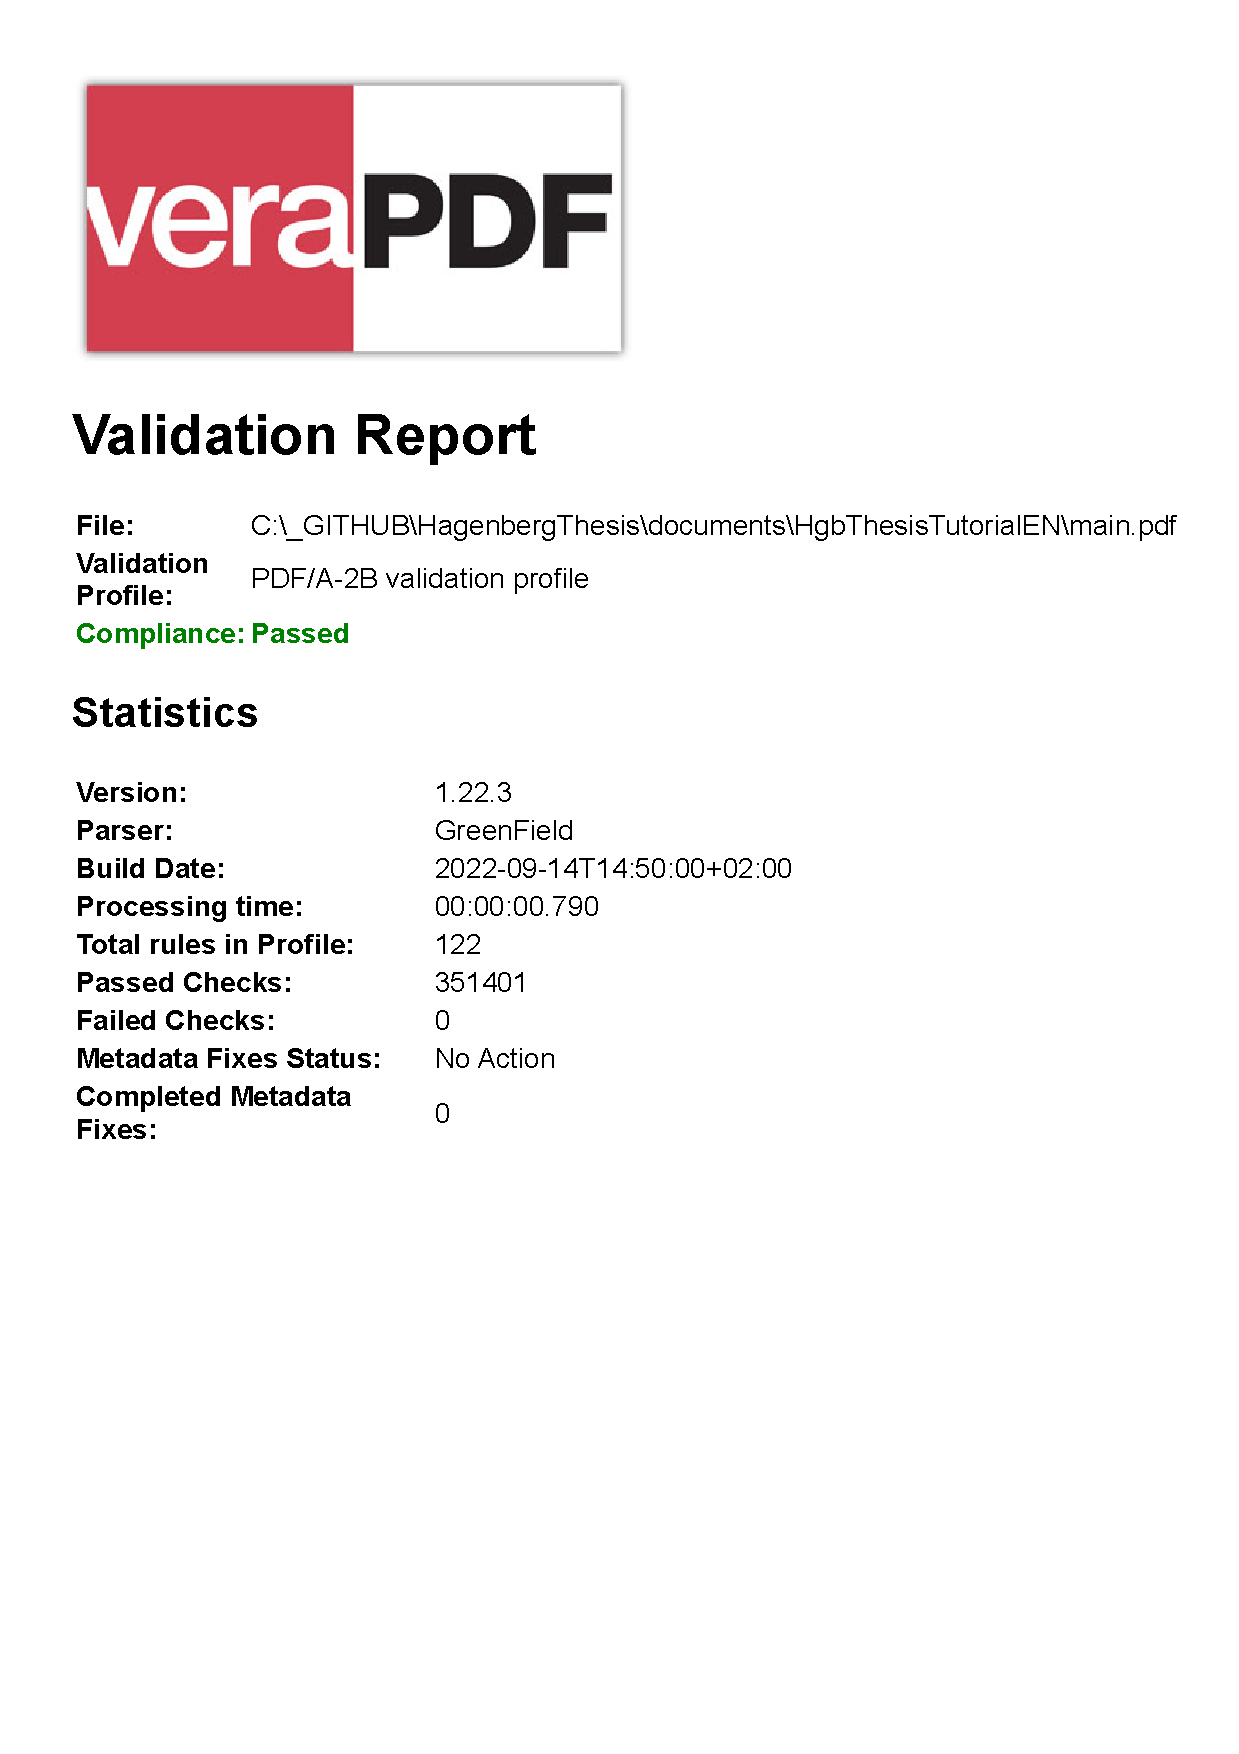
\includegraphics[width=.60\textwidth]{verapdf-report}}
    \caption{Report produced by the \textsf{veraPDF} client after successful validation
    of \emph{this} document. Note that this screenshot was imported as a PDF 
    which itself is \emph{not} PDF/A-compliant.}
    \label{fig:verapdf-report}
\end{figure}


\section{Printing}

Before printing the manuscript, it is advisable to consider a few things in
order to avoid unnecessary trouble (and costs).

\subsection{Digital Submission versus Printing}

For reasons of sustainability, many degree programs no longer require printed
submissions, especially for bachelor's theses. In this case, uploading a PDF
file is sufficient. The declaration is then either signed digitally in the
document or obtained in another way by the degree program. It is advisable to
find out the submission requirements in good time to avoid unnecessary printing
of one's work.

\subsection{Printer and Paper}

If the thesis is printed, this must be done for the final version on a
high-quality \emph{laser printer}; printouts made with inkjet printers are
\emph{not} sufficient. The paper used should also be of good quality (woodfree)
and usual grammage (typ.\ $80\,\mathrm{g} / \mathrm{m}^2$). If only a few
\emph{color} pages are necessary, one may print them separately on a color laser
printer and insert them into the main document (printed in black and white).

By the way, \emph{all} copies to be handed in should be \emph{printed} (and not 
copied)! The cost of printing is no higher than that of copies, but the difference
in quality is---especially for pictures and graphics---usually significant.


\subsection{Print Size}

First of all, make sure that the paper size set in the final PDF file is really
\textrm{A4}! This can be done, for example, with Adobe \emph{Acrobat} or 
\emph{SumatraPDF} via \texttt{File} $\rightarrow$ \texttt{Properties} 
to show the document's paper size:
%
\begin{center}
	\textrm{Correct:} A4 = $8{,}27 \times 11{,}69$ inches or $210 \times 297$ mm.
\end{center}
%
If this does not match, then probably "Letter" is set as the paper size somewhere
in the workflow by mistake.

A common and easily overlooked error when printing PDF documents is caused by 
accidentally setting the "Fit to page" option in the print menu, usually printing 
pages that are too small. Therefore, make sure you check the size of the printout 
by verifying the text width%
\footnote{\Convert[unit=mm]{\the\textwidth}	in this document.} % using 'lengthconvert' package
or using the measurement frame included at the end of this document.
To be on the safe side, this measurement frame should be kept until the work 
is completed, and only then the corresponding page should be removed.
If, as mentioned before, individual color pages are printed separately, these 
should of course also be checked carefully for compliance with the print size!
%\chapter[Closing Remarks]{Closing Remarks%
\protect\footnote{This note only demonstrates the (rarely necessary)
use of footnotes in headings. See the source text for how this is done.
Make sure the footnote does not appear in the table of contents as well!}}%
\label{cha:Closing}

This should be a summary of your thesis, which may also address the
process of its creation, experiences, insights and problems encountered during
the implementation (but no personal issues), areas for improvement, possible
extensions, \etc
Was the topic well chosen, what was eventually achieved,
what points remain open and how could work continue from here?


\section{Read and Let Read}

When your thesis is finished, the first thing you should do is to read it
over again \emph{completely} and \emph{carefully} yourself, even though you
might not feel inclined to once more look at something you have worked on for
so long. In addition, it is highly recommended to have another person do this
as well---you will be amazed at how many additional mistakes you had missed.

The use of AI-assisted writing assistants such as
\emph{Grammarly}\footnote{\url{https://grammarly.com/}} or
\emph{LanguageTool}\footnote{\url{https://languagetool.org/}}
can also be quite useful. However, the suggestions from these tools should not
simply be accepted blindly but with caution.


\section{Checklist}

Finally, Table \ref{tab:checklist} gives a brief checklist of important items
that most frequently are the cause of errors. If an official thesis review is 
required at your university, such and similar items are typically checked 
by the assigned \emph{thesis editor} as well.

\begin{table}
	\caption{List of important items as typically checked during an
	academic \emph{thesis review}.}
	\label{tab:checklist}
	\centering%
	\setlength{\fboxrule}{0.2mm}%
	\setlength{\fboxsep}{2mm}%
	\fbox{%
		\begin{minipage}{0.95\textwidth}
		\begin{itemize}
			\item[$\Box$] \textbf{Title page:}
				length of title (line breaks), name, program of study, date.
			\item[$\Box$] \textbf{Declaration:}
				complete signature.
			\item[$\Box$] \textbf{Table of contents:}
				balanced structure, depth, length of headings.
			\item[$\Box$] \textbf{Abstract/Kurzfassung:}
				precise summary, appropriate length, same content and structure.
			\item[$\Box$] \textbf{Chapter/section titles:}
				length, style, clarity.
			\item[$\Box$] \textbf{Layout/typography:}
				clean printout (no raster fonts), no "manual" spacing between paragraphs or
				indentations, no overlong lines, highlighting, font size, footnote placement.
			\item[$\Box$] \textbf{Language:}
				gender-appropriate wording (no generic masculine or general clause), 
				objective, factual wording.
			\item[$\Box$] \textbf{Punctuation:}
				hyphens and dashes placed correctly, proper spacing after periods
				(especially after abbreviations), correct (front/back) quotation marks.
			\item[$\Box$] \textbf{Figures:}
				quality of graphics and images, font size and type in figures, proper
				placement of figures and tables, captions. Are \emph{all} figures
				(tables) referenced in the text?
			\item[$\Box$] \textbf{Equations/formulas:}
				placement of mathematical elements in continuous text, correct use of
				displayed equations and mathematical symbols.
			\item[$\Box$] \textbf{References:}
				citations properly referenced, including page and chapter references;
				no unresolved cross references (\textbf{??}).
			\item[$\Box$] \textbf{Bibliography:}
				type of publication must be clear in all cases, consistent and complete
				entries, online sources (URLs) cleanly cited.
			\item[$\Box$] \textbf{Other:}
				contents of appendix, PDF
				paper size (A4 = $8.27 \times 11.69$ inches), print size and quality.
		\end{itemize}
		\end{minipage}%
	}
\end{table}




%%%-----------------------------------------------------------------------------
\appendix                                                             % Appendix 
%%%-----------------------------------------------------------------------------

%\chapter{Technical Information}
\label{app:TechnicalDetails}

\section{Current Package Version}

\begin{center}
	\begin{tabular}{@{}ll@{}}
		\toprule
		Date   & File            \\
		\midrule
		\hgbDate & \texttt{hgb.sty} \\
		\bottomrule
	\end{tabular}
\end{center}


\section{Additional Details}

This package is designed for \mbox{UTF-8} encoded source files and supports 
\latex\ in direct PDF mode only.%
\footnote{The "classic" DVI-PS-PDF process is no longer supported.}


\subsection{Technical Requirements}

A current \latex\ installation including
%
\begin{itemize}
		\item \texttt{biber} (modern replacement for BibTeX, Version $\geq 1.5$),
		\item \texttt{biblatex} package (version $\geq 2.5$, 2013/01/10),
		\item Latin Modern fonts (package \texttt{lmodern}).%
			\footnote{\url{https://ctan.org/pkg/lm},
				\url{https://tug.org/FontCatalogue/latinmodernroman/}}
\end{itemize}
%
In addition, a text editor for {UTF-8} encoded (Unicode) files, as well 
as software for opening and viewing PDF files.



\subsection{Use Under Windows}
\label{sec:UseUnderWindows}

A typical installation under Windows looks like this:
%
\begin{enumerate}
\item \textbf{MikTeX}%
	\footnote{\url{https://miktex.org/} -- 
  Generally, the \emph{complete installation} of MikTeX ("Complete MiKTeX") is 
	recommended, as it already contains all necessary additional packages and font files.
	During installation, make sure that the automatic installation of required packages
	is enabled by "\emph{Install missing packages on-the-fly: = Yes}" 
	(NOT "\emph{Ask me first}")!
	It is also recommended to update the installed packages immediately after installing MikTeX 
	and periodically thereafter using the \texttt{MikTeX Console} program.} 
	(basic \latex\ environment),
\item \textbf{TeXstudio}%
	\footnote{\url{https://www.texstudio.org/}}
	(text editor, supports UTF-8 and includes an integrated PDF viewer).
\end{enumerate}
%
Alternative editors and PDF viewers are:
%
\begin{enumerate}
	\item Visual Studio Code%
	\footnote{\url{https://code.visualstudio.com/}}
	with LaTeX Workshop Extension,%
	\footnote{\url{https://marketplace.visualstudio.com/items?itemName=James-Yu.latex-workshop}}
	\item IntelliJ IDEA,%
	\footnote{\url{https://www.jetbrains.com/idea/}}
	with TeXiFy-IDEA plugin,%
	\footnote{\url{https://plugins.jetbrains.com/plugin/9473-texify-idea}}
	\item Lyx,%
	\footnote{\url{https://www.lyx.org/}}
	\item TeXworks,%
	\footnote{\url{https://www.tug.org/texworks/}}
	\item WinEdt,%
	\footnote{\url{https://www.winedt.com/}}
	\item Sumatra PDF ("\latex\ friendly" PDF viewer).%
	\footnote{\url{https://www.sumatrapdfreader.org/}}
\end{enumerate}


\subsection{Use Under macOS}

For macOS, the following configuration is recommended:
%
\begin{enumerate}
\item 
	\textbf{MacTex}%
	\footnote{\url{https://tug.org/mactex/} -- 
	Current MacTeX distributions usually require a mostly up-to-date version of macOS. 
	On older versions, \emph{TeXLive} can alternatively be installed with a special
	installation script. To keep the packages of the \latex\ distribution up-to-date, the 
	\emph{TeX Live Utility} program should be run regularly.}
	(basic \latex\ environment),
\item \textbf{TeXstudio} (text editor, supports UTF-8 and includes an integrated PDF viewer).
\end{enumerate}
%
Alternative editors and PDF viewers are:
%
\begin{enumerate}
	\item Visual Studio Code with LaTeX Workshop Extension,%
	\item Lyx,%
	\item TeXworks,%
	\item Skim ("\latex\ friendly" PDF viewer).%
	\footnote{\url{https://skim-app.sourceforge.io/}}
\end{enumerate}


\subsection{Use Under Linux}

Under Linux the following setup can be used:
%
\begin{enumerate}
	\item 
	\textbf{TeX Live}%
	\footnote{\url{https://tug.org/texlive/} -- An installation under Linux is---depending
	on the distribution used---most easily done with the help of the associated package
	management system (\eg, \texttt{apt-get}).}
	(basic \latex\ environment),
	\item \textbf{TeXstudio} (text editor, supports UTF-8 and includes an
	integrated PDF viewer).
\end{enumerate}
%
Alternative editors and PDF viewers are:
%
\begin{enumerate}
	\item Visual Studio Code with LaTeX Workshop Extension,%
	\item Lyx,%
	\item TeXworks,%
	\item qpdfview ("\latex\ friendly" PDF viewer).%
	\footnote{\url{https://launchpad.net/qpdfview}}
\end{enumerate}


\subsection{Using Online \latex\ Environments}

Besides using a local \latex installation and editor, there are now also good online 
environments that allow to create \latex documents directly in the browser.
The \latex environment is installed on the servers of the provider. Documents can be
created in the online editor or existing templates (such as this document) uploaded and 
edited. Most platforms also allow collaborative work on the same document.

When using such environments, it is highly recommended to perform regular \emph{backups} of your
online data while working, so that in the worst case you don't have to start all over 
again.

\subsubsection{Overleaf}

The most popular editor (tested with this template) is \emph{Overleaf}%.
\footnote{\url{https://www.overleaf.com/}}.
To quickly import template documents from the \texttt{hagenberg-thesis} package, the 
import links in the \emph{readme} section of this project's Github repository%
\footnote{\url{https://github.com/Digital-Media/HagenbergThesis}}
can be used directly.

Please note that free Overleaf accounts have reduced their compile timeouts to only 20 seconds since the end of 2023. This means that larger theses and this template document can no longer be created with it because the PDF generation aborts after 20 seconds.

The only workaround is to purchase a paid account (license) or ditch Overleaf entirely and switch to a local setup. In educational institutions that provide licenses for teachers, they can create a document and share it with students to collaborate, ensuring a smooth workflow.


\subsubsection{Other Online Services}

Besides, there are other online environments for \latex\ and their number is constantly growing, for example:
%
\begin{enumerate}
	\item Papeeria,%
	\footnote{\url{https://papeeria.com/}}
	\item CoCalc.%
	\footnote{\url{https://cocalc.com/}}
\end{enumerate}
 % Technical supplements
%\chapter{Supplementary Materials}
\label{app:materials}


List of supplementary data submitted to the degree-granting institution for archival storage
(in ZIP format).

% Use this as an example only, adapt the structure to your requirements!

\section{PDF Files}
\begin{FileList}{/}
\fitem{thesis.pdf} Master/Bachelor thesis (complete document)
\end{FileList}

\section{Media Files}
\begin{FileList}{/media}
\fitem{*.ai, *.pdf} Adobe Illustrator files
\fitem{*.jpg, *.png} raster images
\fitem{*.mp3} audio files
\fitem{*.mp4} video files
\end{FileList}


\section{Online Sources (PDF Captures)}
\begin{FileList}{/online-sources}
\fitem{Reliquienschrein-Wikipedia.pdf} {\backtrackerfalse\parencite{WikiReliquienschrein2023}}
\end{FileList}




 % Contents of the CD-ROM/DVD
%\chapter{Questionnaire}
\label{app:Questionnaire}





 % Chronological list of changes
%\chapter{\latex-Quellcode}
\label{app:latex}

\section*{Main File (\texttt{main.tex})}

\paragraph{Note:}
This should just be an \emph{example} of how to include source code in the
document's Appendix. It is accomplished with the following instructions:
%
\begin{LaTeXCode}[numbers=none]
\begin{footnotesize}
	\verbatiminput{main.tex}
\end{footnotesize}
\end{LaTeXCode}
%
Of course, the \latex source code of one's thesis is usually \emph{not} 
interesting enough to be reproduced here!

\begin{footnotesize}
	\verbatiminput{main.tex}
\end{footnotesize}





 % Source text of this document

%%%-----------------------------------------------------------------------------
\backmatter                           % Back part (bibliography, glossary, etc.)
%%%-----------------------------------------------------------------------------

\MakeBibliography % References

%%%-----------------------------------------------------------------------------
% Special page for checking print size
%%%-----------------------------------------------------------------------------

\chapter*{Measurement Box}



\begin{center}
{\Large --- Check the size of this box in your printout! ---}

\bigskip

\calibrationbox{100}{50} % Angabe der Breite/Hoehe in mm

\bigskip

{\Large --- Remove this page after printing and checking! ---}

\end{center}



%%%-----------------------------------------------------------------------------
\end{document}
%%%-----------------------------------------------------------------------------
